\section{Введение}

Цель данной главы --- борьба с одним из артефактов восстановления, так называемым эффектом огрубления пучка или Beam Hardening. 
Одна из причин возникночения таких артефактов --- несоответствие излучения реального источника монохроматическому описанию, используемому в моделях для процедуры восстановления.
Другими словами, физическая модель формирования измерений, используемая при восстановлении, не соответствует действительности.
% во-первых, монохроматор, вырезая линию из спектра, сильно уменьшает тем самым интенсивность зондирующего излучения, что в свою очередь влечет за собой увеличение времени измерения. Это минус, а плюс монохроматики состоит в том, что монохроматику можно сфокусировать, а вот с полихроматикой - сложнее. Плюс - хороший монохроматор - это сложная штука сама по себе, его юстировка - серьезная задача, поэтому, если можно обойтись в измерениях без него, то народ обходится.

Для преодоления этого эффекта используют монохроматор - оптический фильтр, вырезающий определенную линию из спектра.
Минусы такого подхода состоят в том, что такой подход сильно уменьшает интенсивность зондирующего излучения, что влечет за собой увеличение времени измерения.
Из плюсов использования монохроматора можно отметить более простую фокусировку рентгеновского пучка.
Само по себе использование монохроматора --- сложная инженерная задача \cite{chukalina2014xray}. 
Качественный монохроматор, который не пропускал бы полихроматическую моду к объекту --- сложный и дорогой прибор. 
Так же является трудной задачей юстировка монохроматора.
Поэтому обычно в реальных измерительных схемах стараются обходиться без использования монохроматора.

При этом обычное ПО восстанавливает характеристику объекта алгоритмами для монохроматического зондирования.
Монохроматический коэффициент поглощения, доставляющий минимум целевой функции, будет содержать артефакты восстановления.
Они образуются из необходимости удовлетворить неправильным ограничениям, возникшим при упрощении физической модели.

Один из способов борьбы с данными артефактами - использование специальных регуляризаций или пост-обработки после восстановления \cite{van2011iterative}.
Другой возможный способ - модифицировать механизм реконструкции таким образом, чтобы процедура находилась в соответствии с более точной физиеской моделью.
В данном случае будет исследована возможность модификации метода восстановления, так, чтобы используемая физическая модель 
В работе восстановление производится в 2D-сечении и задача рассматривается в параллельном пучке.


\begin{comment}
% Томография при Монохроматическом Излучении
% В текущей главе мы представляем алгебраический метод для случая монохро-
% матического излучения. Пусть f(x, y) – восстанавливаемое распределение ли-
% нейного коэффициента ослабления объекта. Пусть на объект падает параллель-
% ный пучок лучей интенсивностью 
%I 0 под углом φ. 
Тогда интенсивность излуче-
ния вдоль некоторого бесконечно тонкого луча со сдвигом s, %l(φ, s)
 после про-
хождения через объект будет
% I(l(φ, s)) = I 0 exp (− ∫ f(x, y)dl).
% (1)
Для краткости записи далее аргументы угла и сдвига, задающие прямую %l(φ, s)

будут опускаться. Данные значения подвергаются нормировке и логарифмиро-
ванию, в результате восстанавливается распределение линейного коэффициента
ослабления для энергии зондирующего излучения, путем решения системы
уравнений:
% ln (I 0 /I(l) ) = p(l) = ∫ f(x, y)dl
для всех углов измерения %φ
 и сдвигов s. Оператор интегрирования вдоль всех
возможных направлений называется преобразованием Радона. При восстановлении реальных измерений как входные данные% p(φ, s),
так и искомая характе-
ристика f(x, y) представляются дискретными изображениями размеров 
%N × M φ и N × N, 
соответственно, а преобразование Радона заменяется на преобра-
зование Хафа.
Для восстановления распределения линейного коэффициента ослабления ис-
пользуются в основном интегральные или алгебраические методы [4]. Особый
интерес представляют последние, так как их, как будет показано ниже, можно
использовать и для восстановления экспериментов, проводимых с использова-
нием полихроматического пучка. Пусть 
%f ∈ R N×N и p ∈ R N×M φ %
– соответ-
ственно входные и выходные данные, H – матрица линейного преобразования
Хафа размера 
%N 3 M φ ≈ N 4
 . Тогда томографическую проекцию можно записать
в виде СЛАУ
%p = Hf.
Решение этой СЛАУ методом наименьших квадратов в явном виде невозможно
ввиду огромного размера матрицы H, однако ее умножение на вектор f, как и
умножение транспонированной матрицы H T может быть посчитано быстро за
O(N 2 log N) используя методы обработки изображений [5]. Применяя метод
градиентного спуска для минимизации L2 нормы расхождения, получаем шаг
градиентного спуска
%f ξ = f ξ−1 + αH T (Hf ξ−1 − p), где
%α - параметр релаксации.
\end{comment}

\section{Модель томографии при немонохроматичесвом излучении}

В реальности спектр используемого для зондирования излучения не сингулярный, а коэффициент ослабления объекта меняется в зависимости от длины волны ($I_0 = I_0(\lambda), f(x, y) = f(x, y, \lambda)$).

Таким образом, при переходе к немонохроматическому случаю, уравнение \ref{eq:mono_fp} принимает следующий вид:

\begin{equation}
\label{eq:white_fp}
I(l) = \int_0^{+\infty}{\left\{
  I_0(\lambda) \exp{\left(-\int{f(x, y, \lambda) dl} \right) d\lambda} 
  \right\}}  
\end{equation}

Таким образом, оператор проецирования становится нелинейным.
При этом в случае, когда источник все же монохроматический, то есть $I_0(\lambda) = \delta(\lambda)$ легко видеть, что уравнение (\ref{eq:white_fp}) переходит обратно в (\ref{eq:mono_fp}).
Спектр используемого в экспериментах источника излучения можно измерить в лабораторных условиях и поэтому считается известным.
Переход к нелинейной задаче не был бы столь существенным, если бы при этом не терялась возможность восстановить зависимость подынтегральной функции от переменной интегрирования. 
Иными словами, без дополнительных знаний о структуре объекта, восстановить искомую функцию $f(x, y, \lambda)$ невозможно.

Предлагается использовать следующую модель формирования функции f %\cite{?}.
Будем считать, что исследуемый объект состоит из смеси K известных элементов, для которых известны их спектральные функции поглощения $f_k(\lambda)$.

Данные функции являются известными величинами, которые можно измерить в лабораторных условиях. В частности в данной работе были использованы значения, возвращаемые функциями библиотеки xraylib \cite{xraylib}.
При этом неизвестными будут пространственные распределения концентрации $c_k(x, y)$ каждого элемента.
\begin{equation}
 \notag
  f(x, y, \lambda) = \sum_{s=1}^K {c_s(x, y) \cdot f_s(\lambda)}
\end{equation}

Учитывая то, что интеграл внутри экспоненцирования – линейный оператор прямой проекции $H$, получим общее значение ослабления интенсивности входного излучения для смеси $c = (c_1, \dots, c_K)^T $ в пикселе измерения $j$ при линейном размере пикслея $\rho$:
\begin{equation}
  \label{eq:white_fp_final}
  I(c)_j = \int_0^{+\infty} {d\lambda \left\{
    I_0(\lambda) \exp{\left(
      -\sum_{k=1}^K {\rho f_k(\lambda) (H c_k)_j} 
      \right)}
  \right\}}
\end{equation}

Далее будет предложен итерационный процесс восстановления концентраций $с_k$, основанный на алгебраическом методе и минимизации $L_2$-нормы.

\section{Алгебраический метод для немонохроматического случая}

В финале раздела будет выведена формула для расчета поправки на каждом шаге итерации метода восстановления концентраций $c_k$.
Пусть далее $i$ индексирует пиксели в пространстве исходных изображений-концентраций размера $N \times N$, $j$ индексирует пиксели в пространстве входных изображений-измерений размера $N \times M_\varphi$, а $k$, как и раньше, принимает значения $1 \dots K$ и индексирует различные элементы, составляющие исследуемый объект.
Пусть $h_{ij}$ – элементы матрицы прямой томографической проекции H.
Обозначим так же значения, измеренные детектором за $t$

Для того, чтобы выписать минимизационную процедуру необходимо составить функцию невязки.
По аналогии с выводом итерации алгебраического метода для монохроматичного случая, можно взять квадратичную невязку вида $(I(c) - t)^2$.
Однако эта величина размерная и зависит от суммарной мощности просвечивающего пучка.
Поэтому предлагается минимизировать невязку нормированных интенсивностей на величину $ S = \int_0^{+\infty}{I(\lambda)d\lambda}$.
Итак финальная функция для оптимизации имеет вид:
\begin{equation}
\label{eq:white_cost_function}
Q(c) = \left(\frac{I(c) - t}{S}\right)^2,
\end{equation} 
где за возведение в квадрат подразумевается обычная эвклидова норма разницы векторов размера $N \times M_\varphi$.

Для того, чтобы выстроить итерационный процесс вычисления концентраций, необходимо подсчитать градиент весовой функции по концентрациям каждого из элементов. 
Сделаем это покомпонентно:
\begin{equation}
  \notag
  \frac {\partial Q_j} {\partial c_{ki}} = 
  2 \frac {(I(c) - t)_j} {S} 
  \frac {\partial } {\partial c_{ki}}
  \left( \frac {I(c)_j} {S} \right).
\end{equation}

Рассчитаем возникшую частную производную:
\begin{equation}
  \notag
  \begin{split}
  \frac 1 S
  \frac {\partial I(c)_j} {\partial c_{ki}} &= 
  \frac 1 S
  \int_0^{+\infty} {d\lambda \left\{
    I_0(\lambda) 
    \frac \partial {\partial c_{ki}}
    \exp{\left(
      -\sum_{s=1}^K {\rho f_s(\lambda) (H c_s)_j} 
      \right)}
    \right\}} = \\
  &= 
  \int_0^{+\infty} {d\lambda \left\{
    -\rho f_k(\lambda) 
    \frac {I_0(\lambda)} {S}
    \exp{\left(
      -\sum_{s=1}^K {\rho f_s(\lambda) (H c_s)_j} 
         \right)}
    \frac {\partial (H c_k)_j} {\partial c_{ki}}
    \right\}} = \\
  &= 
  \frac {\mu_{kj}} {S} \frac {\partial (H c_k)_j} {\partial c_{ki}},
  \end{split}
\end{equation}

где введено обозначение $\mu_k$ для весовых коэффициентов, имеющих размерность синограммы и зависящих от элемента и прямой проекции:

\begin{equation}
  \label{eq:weights}
  \mu_{k} = \int_0^{+\infty} {d\lambda \left\{
    -\rho f_k(\lambda) 
    I_0(\lambda)
    \exp{\left(
      -\sum_{s=1}^K {\rho f_s(\lambda) (H c_s)} 
         \right)}
    \right\}}
\end{equation}

Эти коэффициенты должны учитывать спектральное взаимодействие различных элементов с источником, взвешивая невязку для каждого элемента, благодаря чему на каждой итерации вклад в разные концентрации будет разный.

Заметим, что производная $\frac {\partial (H c_k)_j} {\partial c_{ki}}$ соответствует обратной проекции в алгебраической процедуре восстановления. 
Таким образом, шаг итерации будет иметь вид
\begin{equation} \label{eq:part3_whitegrad}
  \nabla_k \ Q = 2H^\intercal R_k \text{, где } R_{kj} = \frac {(I(c) - t)_j} {S} \mu_{kj}
\end{equation}

Где за $R_k$ обозначена взвешенная невязка для элемента $k$. 
Таким образом, мы вычислили компоненты градиента по каждому из составляющих исходный объект элементу.
Как видно из формулы \ref{eq:part3_whitegrad}, компоненты градиентов по различным элементам могут вычисляться отдельно.
Тем не менее, не стоит забывать, что все элементы связаны через взвешенные невязки $R_k$ , в которых содержится зависимость от всего вектора $c$.
Итак, наконец, шаг итерации алгоритма выглядит следующим образом:
\begin{equation}
  \label{white_iteration}
  c_k^\xi = c_k^{\xi - 1} - \gamma_k (\xi - 1) H^\intercal R_k(c_k^{\xi - 1}).
\end{equation}

\section{Численный Эксперимент} \label{sect_3_2}
Одним из результатов данной главы является программная реализация и исследование работы алгоритма восстановления, основанного на взешенных невязках.
Алгоритм был реализован на языке python с использованием библиотеки ASTRA \cite{van2015astra}.
Для восстановления были использованы модельные данные (фантом), состоящий из двух овальных областей, имеющих пересечение и состоящих из элементов номер 22 и 28.
Распределения концентраций элементов представлены на рисунке \ref{fig:white_phantom}

%\begin{figure}
%\begin{subfigure}[h]{0.45\textwidth}
%  \centering
%    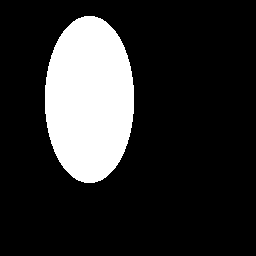
\includegraphics[width=\textwidth]{part3_img/c_22}
%  $c_22$
%\end{subfigure}
%\begin{subfigure}[h]{0.45\textwidth}
%  \centering
%    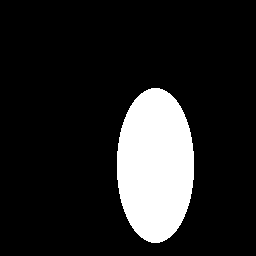
\includegraphics[width=\textwidth]{part3_img/c_28}
%  $c_28$
%\end{subfigure}
%  \caption{Используемые для симуляций концентрации}
%\label{fig:white_phantom}
%\end{figure}

\begin{figure}
  \centering
\begin{tabular}{@{}c@{}c}
    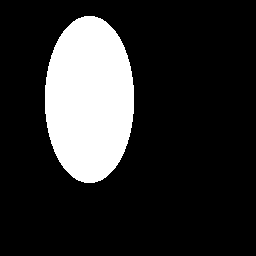
\includegraphics[width=0.45\textwidth]{part3_img/c_22}
  &
    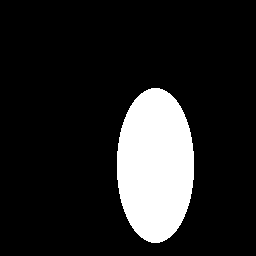
\includegraphics[width=0.45\textwidth]{part3_img/c_28}
  \\
    $c_22$ & $c_28$
\end{tabular}
  \caption{Используемые для симуляций концентрации}
\label{fig:white_phantom}
\end{figure}


На рисунке \ref{fig:source} представлены спектры поглащения элементов и спектр испускания выбранного для симуляций источника.

\begin{figure}
  \centering
  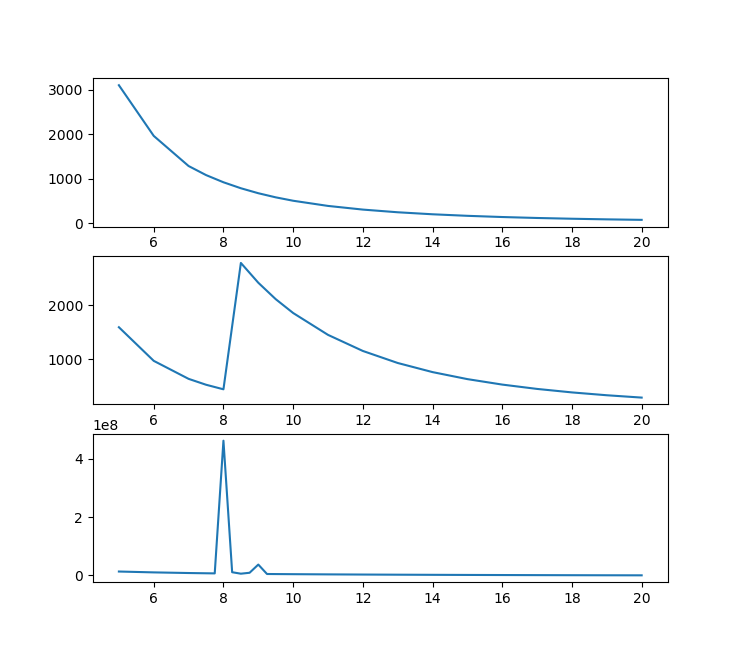
\includegraphics[width=0.95\textwidth]{part3_img/graphs}
  \caption{Сверху вниз: коэффициент поглощения для элементов 22, 28 и спект источника}
  \label{fig:source}
\end{figure}

При проведении первых симуляций оказалось, что восстановление итерационными методами сходится к локальному минмуму мультиспектральной задачи.
Это проявляется в том, что промежуточные концентрации в результате градиентного спуска приходят в вырожденному решению, не содержащему специфики элементов, из которых состоит образец.
Обе концентрации получаются равномерно размазанными по площади, занятой объектом, с характерными артефактами --- лишним увеличением концентрации вдоль выпуклой оболочки \ref{fig:wrart_noreg_25}.
Вырождение состоит в том, что значения концентраций отличаются в константу раз равномерно по всей площади восстанавливаемых концентраций.

\begin{figure}
  \centering
  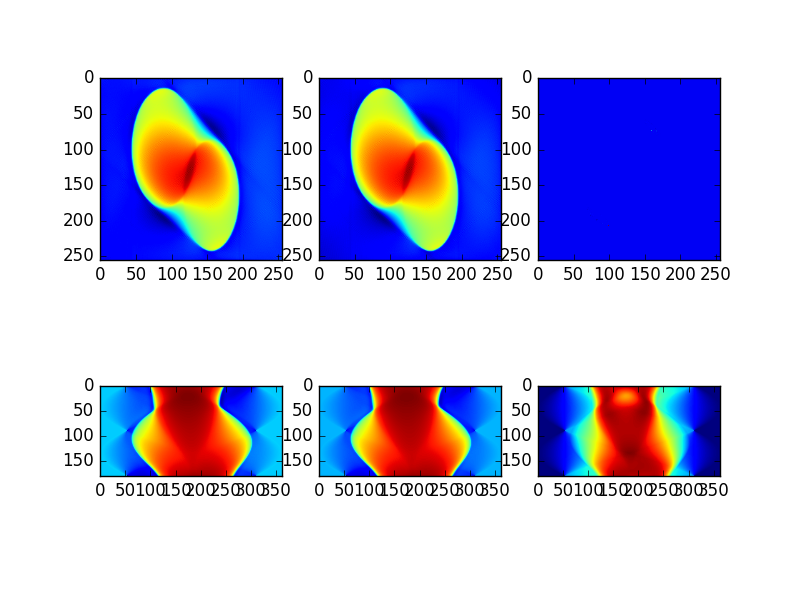
\includegraphics[width=0.95\textwidth]{part3_img/no_reg_iteration_25}
  \caption{Восстановление с помощью МВН, концентрации и их отношение, их синограммы и отношения}
  \label{fig:wrart_noreg_25}
\end{figure}

\todo{вывести соотношение, к которому выраждаются восстановленные картины}

\section{Полихроматическая регуляризация}
\todo{описать подробно регуляризацию модуля произведений}

Вырождение концентраций различных элементов легко проиллюстрировать следующим примером.

\todo{сингулярный спектр, сингулярные кривые поглащения двух элементов. реконструкция - решение уравнения с 2 неизвестными. график в координатах c1, c2, решение лежит на отрезке между осями в положительном квадранте (для некоторого пикселя). вырождение идет к прямой $c_1 = \alpha c_2$. Нужно запретить это - одновременно нельзя обеим концентрациям быть положительными. Иными словами, $c_1 c_2 = 0$}

Логичным ограничением при оптимизации является запретить находиться в одном пикселе восстанавливаемой площади концентраций двух разных элементов.
Чтобы ввести такое ограничение, можно перейти к задаче условной оптимизации, добавив ограничение $c_1 c_2 = 0$ или, в случае $K$ различных элементов $\frac{ K (K - 1) } { 2 }$ ограничений вида $c_{k_1} c_{k_2} = 0, k_1 \neq k_2$.
Так же можно добавить условия на положительность концентраций $c_k \geq 0$.
В результате восстановление томографии в полихроматической моде сведется к оптимизации с ограничениями.
Следуя логике раздела \ref{sect_2_2}, заменяя жесткие ограничения-равенства на мягкие, получаем что регуляризация может быть получена добавлением в целевую функцию штрафов за модуль произведения концентраций. 
Дополнительно добавляется мягкий штраф за отличие значений концентраций от 0 и 1, подобно тому как это сделано в \cite{svets2016}: $||c - 0.5||^2$
\todo{описать подробнее}

Результаты восстановления с использованием такой мультипликативной регуляризации (мягких ограничений-равенств условной оптимизации) представлены на рисунке \ref{fig:wrart_mulreg_150}

\begin{figure}
  \centering
  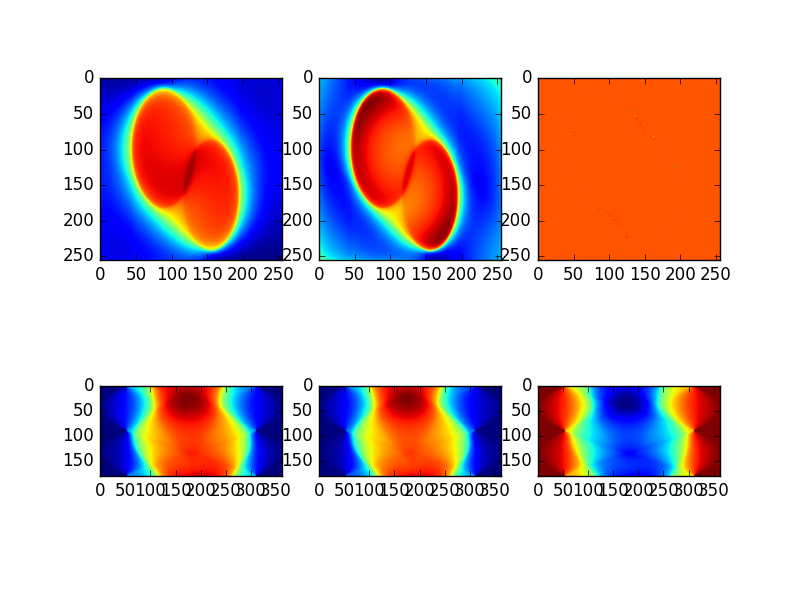
\includegraphics[width=0.95\textwidth]{part3_img/mul_reg_iteration_150}
  \caption{Восстановление с помощью МВН с использованием мультипликативной регуляризации}
  \label{fig:wrart_mulreg_150}
\end{figure}

\todo{описать переход к вырожденному спектру}

\section{Выводы} \label{sect_3_3}
